\documentclass[compress]{beamer}

\usepackage{beamerthemesplit}
\usepackage[german]{babel}
\usepackage{ucs}
\usepackage[latin9]{inputenc}
\usepackage{graphicx}
\usepackage{multirow}

\usetheme{Frankfurt}
\usecolortheme{default}

\title{PM Lab Tools}

\author{Johannes Wei�, Jonathan Dimond}

\date{\today}

\begin{document}

\frame{\titlepage}

\section{Outline}

\frame {

  \frametitle{Outline}

  \begin{itemize}

  \item Basics

  \item Programmatic C API (a.k.a. \texttt{libpmlab})

  \item Stream Based Plain Text Data (a.k.a. \texttt{pmclient})

  \item Real--time Data Viewer (a.k.a. \texttt{realtime.py})

  \end{itemize}

}


\section{Basics}

\subsection{GIT Repository}

\frame {

  \frametitle{\texttt{git} Repository}

  \texttt{\$ git clone git://github.com/weissi/pm-lab-tools.git}

  \texttt{\$ cd pm-lab-tools/client}

  \texttt{\$ ls}

  \texttt{libpmlab.h \# Programmatic C-API}

  \texttt{libpmlab.c \# Programmatic C-API}

  \medskip{}

  \texttt{pmlabclient.c \# Stream Based Plain Text Data}

  \medskip{}

  \texttt{realtime.py \# Real--time Data Viewer}

  \medskip{}

  \texttt{sample.R \# R sample}

  \texttt{sample.gp \# gnuplot sample}
}


\subsection{Building}

\frame {

  \frametitle{Building}

  \texttt{cd pm-lab-tools}

  \texttt{./build.sh client}

  \bigskip{}

  \texttt{build/pmlabclient i30pm1 12345 pmX \# Execute}

}


\section{Programmatic C API}

\begin{frame}[fragile]

  \frametitle{Programmatic C API}

\begin{verbatim}

void *pm_connect(char *server,
                 char *port,
                 unsigned int *channels,
                 unsigned int num_channels);


int pm_read(void *handle,
            size_t buffer_sizes,
            double *analog_data,
            digival_t *unused,
            unsigned int *samples_read,
            uint64_t *timestamp_nanos);

void pm_close(void *handle);
\end{verbatim}

\end{frame}


\section{Stream Based}

\begin{frame}[fragile]

  \frametitle{Stream Based Plain Text Data}

\begin{verbatim}
$ build/pmlabclient localhost 12345 | head
40221.000000 0.023850 0.023165 0.023238 0.000482 0.003031 0.006778
40221.000056 0.024285 0.023034 0.022915 0.002563 0.002781 0.004928
40221.000111 0.024726 0.023468 0.023225 0.002860 0.002827 -0.002475
40221.000167 0.023791 0.023053 0.024166 0.003097 0.002853 -0.004155
40221.000222 0.023732 0.023238 0.023132 0.002056 0.003242 0.002313
40221.000278 0.024298 0.022895 0.023145 0.002570 0.001332 0.005613
40221.000333 0.024496 0.023086 0.023099 0.002590 0.002972 0.003578
40221.000389 0.024094 0.023475 0.023883 0.002418 0.002385 -0.005459
40221.000444 0.023811 0.023238 0.022941 0.003452 0.003413 -0.001514
40221.000500 0.024199 0.023139 0.023185 0.002003 0.003044 0.006759
\end{verbatim}

\end{frame}


\section{Real--time Viewer}

\begin{frame}

  \frametitle{Real--time Viewer}

\texttt{build/pmlabclient localhost 12345 | \\}
\texttt{    client/realtime.py 10}

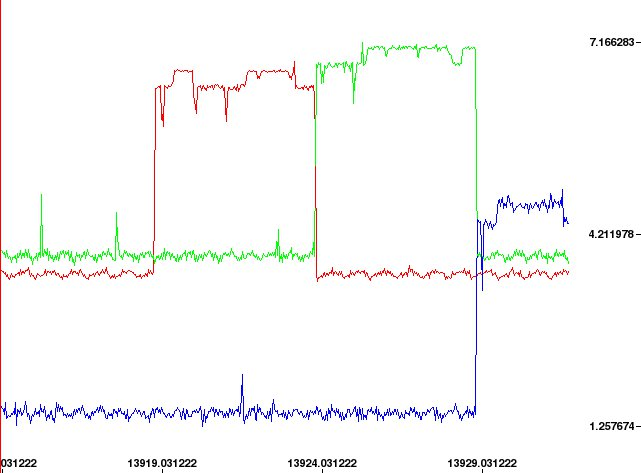
\includegraphics[width=7cm]{pm-5-6-7-power.jpg}

\end{frame}


\end{document}
% vim: set spell spelllang=en_us fileencoding=latin9 : syntax spell toplevel :
